 \documentclass[12pt]{amsart}
 \usepackage[margin=1in]{geometry}                % See geometry.pdf to learn the layout options. There are lots.
 \geometry{letterpaper}                   % ... or a4paper or a5paper or ... 
 %\geometry{landscape}                % Activate for for rotated page geometry
 %\usepackage[parfill]{parskip}    % Activate to begin paragraphs with an empty line rather than an indent
 \usepackage{graphicx}
 \usepackage{url}
 \usepackage{color}
 \usepackage{amssymb}
 \usepackage{xfrac}
 \usepackage{epstopdf}
 \usepackage{siunitx}
 \usepackage[]{natbib}
 \usepackage{textcomp}
 \usepackage{multirow}
 \usepackage{threeparttable}
 \usepackage{setspace}  % Needed for Double Spacing
 \usepackage[english]{babel}
 \usepackage{soul}
 \usepackage{microtype}
 
 %Approx Tilde
 \newcommand{\textapprox}{\raisebox{0.5ex}{\texttildelow}}
 
 
 \DeclareGraphicsRule{.tif}{png}{.png}{`convert #1 `dirname #1`/`basename #1 .tif`.png}
 
 \title[Logical Circuitry using SiC for Control in Harsh Environments]{Development of Logical Circuitry using Silicon Carbide Substrates for Control Circuits in Harsh Environments}  % add title here
 \author{Wesley T. Honeycutt}  % include Author's name here
 %\date{}                                           % Activate to display a given date or no date
 
 \begin{document}
 	\maketitle
 	
 	\doublespacing
 	
 	
 	\noindent
 	\textbf{Title of Research Opportunity}: \textsc{SiC Circuit and Device Design and Fabrication}\\
 	\smallskip
 	\noindent
 	\textbf{NASA Center}: \textsc{Glenn Research Center}\\
 	\smallskip
 	\noindent
 	\textbf{NASA Advisor}: \textsc{Gary W. Hunter and Phil Neudeck}\\
 	\smallskip

 	\section{Statement of problem}
 	
 	Recently, NASA has begun prioritizing an exploratory mission to Venus~\cite{herrick2014goals}, including a surface lander~\cite{kremic2017long}.  Previous landers from the Venera program by the USSR were only able to last, at most, two hours on the unforgiving Venusian surface~\cite{hunten1983venus}.  The extreme temperatures and oxidative atmosphere of the planet's surface mean it is very difficult for current electronic systems to perform for extended periods.  While a wealth of new high temperature and pressure sensing instruments have been developed as part of the Venus Exploration Analysis Group (VEXAG), the glue electronics to control and operate such a lander are still elusive~\cite{balcerski_venus_2015}.  
 	
 	The development of silicon carbide (SiC) semiconductor devices has gained increasing popularity in the past 20 years, yet the technology lacks the wide breadth of available devices which competing substrates currently offer.  Far from the first light emitting diode~\cite{round_note_1907,losev_luminous_1927} which was originally made in SiC, today SiC can be found in many high power applications.  Recent developments have even allowed the creation of power switching devices with high-voltage junction temperature tolerance up to \SI{1200}{\volt} in both JFET and MOSFET designs~\cite{siemieniec_1200v_2011,mino_gate_2003}.  Current SiC logical devices are produced using JFET technology.  Core logic gates such as the inverter, NAND, and NOR have been demonstrated in both depletion mode~\cite{krasowski_n_2010} and enhancement mode~\cite{habib_complementary_2013} SiC JFET.  Despite recent demonstrations of a ring oscillator~\cite{whate} and development of 100's scale transistor level logic using SiC JFET technology~\cite{neudeck_first-order_2016}, there is a dearth of advanced logic designs for SiC circuits which would further the NASA Venus lander objectives.  The goal of this proposed work is to develop discrete digital logic devices using SiC substrates and patterning. 
    
 	
 	%\begin{figure}[htbp] %  figure placement: here, top, bottom, or page
 	%   \centering
 	%   \includegraphics[width=2in]{example.jpg} 
 	%   \caption{example caption}
 	%   \label{fig:example}
 	%\end{figure}
 	
 	\section{Background and relevance to previous work}
 	
 	Silicon carbide has several interesting properties that make it an attractive semiconductor platform for devices intended to withstand harsh environments.  At standard atmospheric pressures, SiC remains crystalline with no defects at temperatures up to \SI{2760}{\degreeCelsius} before partial sublimation~\cite{haase_si-c_1985}.  At higher pressures, this temperature stability increases.  Under 100 atm, similar to the pressure at the surface of Venus, SiC remains solid up to \SI{2830}{\degreeCelsius} before melting.  Individual junctions of p-doped and n-doped SiC material have a much higher tolerance for heat than more commonly used substrates such as Si.  This is because the optimum working temperature of SiC is very close to the highest normal mode vibrational temperature, or band gap~\cite{chelnokov_high_1997}.  Microelectromechanical systems (MEMS) based on SiC have been established as a viable device for some time~\cite{sarro_silicon_2000}, and some developed MEMS devices are pushing temperature limits in sensors~\cite{okojie_zero_2010}.  Logic gates manufactured from SiC can take advantage of this property by creating devices which tolerate high voltage switching, a task which produces a large amount of heat~\cite{weitzel_silicon_1996}.  The converse can be true as well: it is possible to make low power logic gates that tolerate extreme temperatures.   
 	
 	Additionally, SiC has been shown to be particularly resilient against radiation damage.  Circuits made of SiC have been reported to exhibit much lower rates of carrier damage due to deep material defects caused by neutron flux, with McGarrity et al. reporting \sfrac{1}{3} of the damage compared to Si based devices at doses of $10^{16}$~neutrons/$cm^2$~\cite{mcgarrity_silicon_1992-1}.  This makes SiC technology attractive for radiation heavy environments, including satellites and exploratory vehicles.  The large gate sizes in current SiC technology compared to modern CMOS feature sizes makes the SiC further resistant to radiation effects~\cite{zhou2004transistor}.  If this material is used for the sensitive electronic equipment, it is possible to have reduced failure rates with current design specifications.  Furthermore, it is possible that future devices using this technology may require less device redundancy for radiation hardening purposes, making it possible to create exploratory vehicles with greater computational power and reduced power consumption.  
 	
 	Logical units for SiC are designed by the NASA Silicon Carbide Electronics and Sensors group using depletion mode JFET technology on both 4H-SiC and 6H-SiC wafers.  At the simplest level of description, an n-type JFET, the most durable and stable type for high temperature operation~\cite{neudeck_first-order_2016}, is a transistor gate with the drain and source connected to an n-type substrate with a p-type gate separated by a depletion layer.  A detailed diagram of the current archetypal SiC JFET layers can be found in the literature~\cite{neudeck2016first}.  These JFETs are normally ON devices which switch OFF when a voltage applied to the gate passes a certain threshold in a reverse biased regime.  Due to this design, the source requires a negative voltage, making the HIGH and LOW bits ground and a negative voltage, respectively.  As certain parts of a logical array require a positive voltage, a JFET logic circuit is necessarily more complex to design due to the presence of an additional power rail.  Further complications arise from the body bias effect based on the substrate voltage~\cite{neudeck2015experimental} and radially dependent resistivity observed in printed wafers~\cite{neudeck2016first}.  
 	
 	As a physical chemist, I have an outside perspective on device function at the gate interface level which allows for a critical approach to the challenges posed by innovative logic design.  My previous experience with silicon based control systems has demonstrated that I am capable at computer aided design (CAD) of electronic systems~\cite{honeycutt_development_2017}.  In addition to my design experience, I have also used modeling programs such as SPICE to characterize the behavior of a Fourier transform device for monitoring sample conductivity.  Modern developments in microcontroller prototyping boards allow for integration of one device to test another.  My previous work gave me experience with prototype evaluation of electronic systems and bringing a scientific approach to an engineering problem.  Particularly, previous designs for sensors deployed in unpredictable climates have made me conscious of the need for devices built to tolerate these conditions including temperature dependent conductivity sensors~\cite{honeycutt_comparison_2017}.  As a scientist who enjoys developing devices for monitoring and evaluating physical and chemical properties, the challenges posed by SiC JFET design appeal to my desire to broaden my skills.
 	
 	\section{General methodology, procedures to be followed, and timeline for completion of each step}
 	\label{sec:methods}
 	
 	The goal of this proposed work is to develop logic circuits required for a low power monitoring device tolerant to harsh conditions by application of known computing architecture to the emerging silicon carbide technology.  At the highest level of abstraction, a device of this nature requires a central processing unit (CPU), level shifters, analog to digital converters (ADC), switched power supply units (PSU), and memory.  Certain portions of this list, including level shifters~\cite{krasowski_n_2010}, ADC~\cite{hedayati2016500}, and PSU~\cite{kargarrazi_500_2015}, have been demonstrated in previous research. In the case of a modern application, a single package microprocessor can handle most of these tasks.  However, minimal work has been done creating complex logic for the CPU in SiC.  The development of this device must start from a basic level, designing the subcomponents of the CPU individually.  
 	
 	A CPU can be generalized as a combination of individual logic units, primarily these are registers and arithmetic logic units (ALU).  The goal of this proposal is to develop the technology in SiC JFET for both of these logic units to create a functional 8-bit microprocessor.  
 	
 	\subsection{Register}
 	
 	The register is a logic unit which is included in many important CPU and device components such as the primary register, memory, instruction set, and program counter.  To construct this unit, we must reduce this piece down to its relatively simpler components.  The register is a series of clock synchronized flip-flops, a flip-flop is a pair of latches, a latch is simply a pair of NOR gates connected in a certain manner, and a NOR gate is constructed from a few individual transistors.  Figure~\ref{fig:register} shows the decreasing levels of abstraction from the register of a popular integrated circuit to the layers and doping of a single NOR gate designed for CMOS technology.  The transistor technology for JFET SiC gates have been previously demonstrated for NOR gates, making the technology scale up possible. 
 	
 	 	\begin{figure}[htbp] %  figure placement: here, top, bottom, or page
 	 	   \centering
 	 	   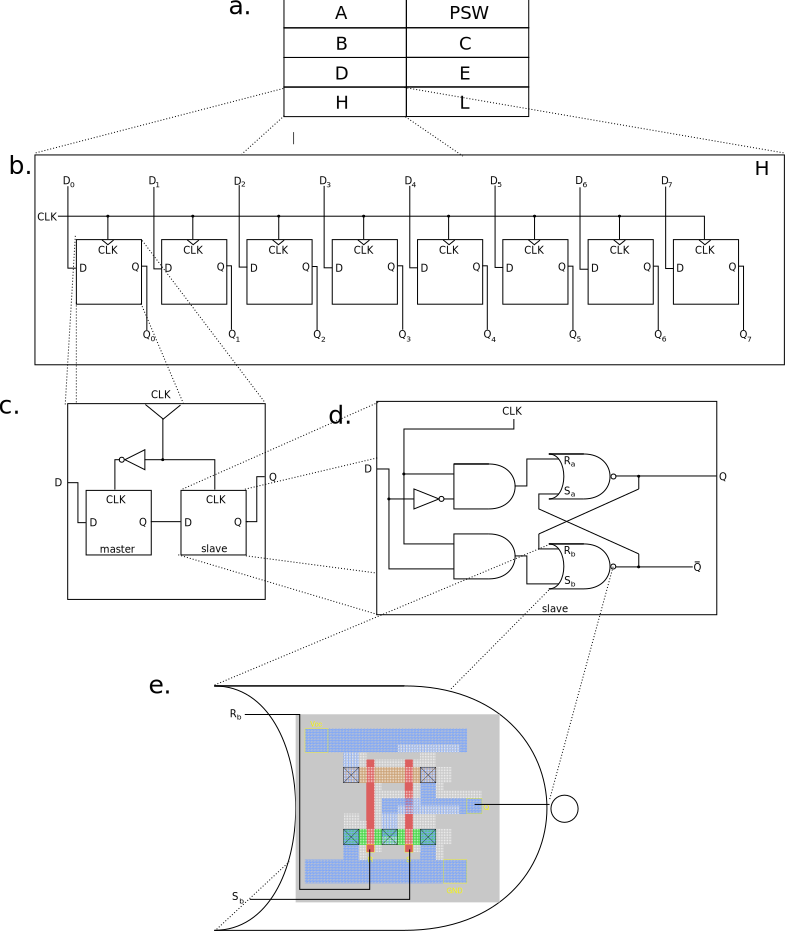
\includegraphics[width=.8\columnwidth]{register.pdf} 
 	 	   \caption{This is an example register design showing the design hierarchy.  Part~$a$ shows the primary user accessible 8-bit registers included in the design of the popular Intel 8085 chip~\cite{intel_corporation_8080/8085_1978}.  Part~$b$ shows detail of one register from part~$a$~\cite{harris_digital_2012,patterson_computer_2013}.  Each bit of the register is a flip-flop which adjusts the value from D to Q for each bit on in a clock cycle.  Part~$c$ shows one of these flip-flops.  A flip-flop is composed of two latches, a master and a slave, which copy D to Q on the rising edge of the clock cycle.  This saves the state of the flip-flop at all other times.  Part~$d$ shows one of the latches, a simple logic circuit consisting of one NOT, two ANDs, and two NORs in a bistable arrangement.  Part~$e$ shows a diagram of one CMOS NOR gate depicted in part~$d$ as they would be designed for patterning on the SiC surface using the program MAGIC~\cite{ousterhout1985magic}.  In short: multiple of $e$ make up $d$, which make up $c$, which make up $b$, which make up $a$.}
 	 	   \label{fig:register}
 	 	\end{figure}
 	 	
 	
 	Due to the synchronous nature of the register and the importance of timing in computing, each device will be rigorously analyzed as it is created and tested.  As it is impractical to directly measure single gate delay, a value which is often on the scale of picoseconds, it is useful to estimate the rise and fall of a signal through a gate using computational models and values of capacitance and current for each interconnect~\cite{kaushik_waveform_2007}.  The delay for multiple equivalent gates is additive at scale, making the averaged delay over multiple gates in a device a calculable quantity with simple instrumentation.  The averaged gate speed can be measured by construction of an array of latches acting asynchronously.  This will be used to verify computationally calculated values. 
 	
 	Keeping with the ``bottom-up'' approach to design on the SiC substrate, the first task will be designing and verifying a single bit flip-flop, which has not been reported in literature.  The patterned device will be characterized by tests to determine the ability to retain and replace the bit over multiple clock cycles.  As SiC devices are being sought to operate in harsh conditions, tests will be undertaken to determine the bit retention ability of the flip-flop at a range of temperatures from standard conditions to \textgreater\SI{500}{\degreeCelsius}.  Testing of the device can take place with a voltage monitor (capable of determining bit state) at short time scales and a local RC oscillator (as oscillators must be close to the circuit to prevent return current, making an external crystal oscillator impractical for high temperature tests).  The second task will be to scale this device up to a full 8-bit register.  Findings from the first task will be used to determine the design of this circuit, and it will be tested and verified in a similar manner.
 	
 	\subsection{Arithmetic Logic Unit}
 	
	Another essential component of the CPU is the Arithmetic Logic Unit (ALU).  This is an umbrella term for portion of the processor which performs simple arithmetic operations such as addition, subtraction, multiplication, division, and comparison.  Each of these operations requires a distinct circuit.  The addition and subtraction circuitry will be designed in the form of a carry-lookahead adder (chosen for the ability to perform faster calculations than many other adder circuits, a property which will be valuable in lifetime-limited missions), using two's compliment values for subtraction operations.  The multiplication and division operations will be performed on circuitry designed using logical and arithmetic shifters.  Equality comparators are simple ANDs of a number of XNOR gates, which can be constructed from the NAND and NOR gates available in SiC JFET.  Magnitude comparators are a variant of subtractors.  All of these have well documented logical designs which can be applied to SiC systems.
	
	Simple arithmetic circuits are used throughout the computer system.  For example, operations are performed based on orders delivered by Operation Codes (Opcodes) from the program register.  These instructions must be interpreted by the logic of the device by arithmetic means.  For example, an adder is used to determine the address of the next instruction from the program counter, and a control ALU is utilized to compute the memory address of data to be operated upon by the CPU.  With a working register established, it will be necessary to develop a way to utilize the register directly by furnishing it with operations.  The development goal of designing a working ALU furthers the overarching goal of creating a working processor, as the individual components of the ALU are used in many places.  
	
	The first task of the ALU portion of this proposal is to demonstrate a simple half-adder circuit patterned in SiC.  The half-adder will be fed alternating values of HIGH and LOW on both inputs to determine if a correct value is generated for the output and/or the carry of the circuit.  The input for this circuit will be generated by an external microcontroller such as an Arduino prototyping board timed to send the signal pulses at regular intervals and check the answers.  The Arduino will log the inputs, output, and carry from this circuit to check for errors.  This experiment will be repeated in both standard conditions and harsh conditions in excess of \SI{500}{\degreeCelsius} to simulate real operation.  The Si based Arduino signal generation and logging can be isolated from the elevated temperature conditions since HIGH and LOW signals are not subject to the same trace length constraints as oscillators.  Success of the circuit will be determined by continuous operation without errors with a lifetime to match previously explored logical units~\cite{spry2016processing}, discussed further in Section~\ref{sec:results}.  The next task will be to scale up to an 8-bit full adder, then to a carry-lookahead adder which will be tested in the same manner.  
	
	Comparators and shifters will be tested in a similar ``bottom-up'' manner and constraints as the adder.  For the comparator, initial tests will be performed on a simple 2-bit comparator, then scaled up to a full 8-bit comparator.  The first bit shifter will be a simple array shifter of 2-bits, tested by cycling the bit shift by one unit over time.  The scaled up version of the shifter will be tasked with performing full 8-bit shift operations.  Tests will be performed at a range of temperature conditions and deemed successful for continuous operation without errors, similar to the other proposed units of the ALU.
 	
 	\section{Explanation of new or unusual techniques}
 	
 	The proposed work is unique in that it uses SiC for logical device fabrication.  There are very few devices which use this technology, and use of substrate materials outside of Si in CMOS design is uncommon due to industry focus on small feature sizes and high computational power.  While this is a new and exciting area of research, there will be few novel techniques implemented at this stage.  The design flow for computers at the Si level is so well documented that many university level research institutions offer courses on the most up-to-date processes available.  However, the technology for SiC devices is young compared to Si devices, many of these modern methods make use of architecture and design technology not prepared for the simplicity of SiC.  Therefore, a ``back-to-basics'' approach is more suitable for this project.  The ``back-to-basics'' approach will favor the use of the original VLSI work pioneered by Mead and Conway, and their contemporaries~\cite{mead_introduction_1980,pucknell_basic_1988,slater_microprocessor-based_1987}.
 	
	While much of the design for modern integrated circuits is handled by computational algorithms, few such mathematical models are available for the SiC substrate.  The current state of circuit simulation makes use of NMOS SPICE models with certain parameters ignored~\cite{neudeck_first-order_2016}.  Instead, a more traditional approach to device design must be considered.  Masks for experimental devices will require manual generation based on traditional standard for VLSI device production pioneered by Mead and Conway~\cite{mead_introduction_1980}.  Previous work by the SiC group at NASA has produced some important values for device modeling including size constraints.  Physical constants observed in this work will be used to further develop a custom technology profile for SiC in a VLSI design program such as MAGIC~\cite{ousterhout1985magic}.  By recording these parameters, it is possible to approach the algorithmic simplicity enjoyed by traditional substrate devices, establishing Electronic Design Automation (EDA).  The modularity and regularity inherent to the nature of computer design makes these values extremely valuable as the overarching project scales up.  Furthermore, VLSI EDA programs can be used in conjunction with SPICE to simulate the designed circuits at the pattern level~\cite{Nagel:M382}.  
 	
 	\section{Expected results and their significance and application}
 	\label{sec:results}
 	
	The qualifications for an individual circuit success were previously mentioned in Section~\ref{sec:methods}.  Generally, these success criteria can be divided into data retention time for register devices and continuous error-free operation time for ALU related devices.  Some electronic properties are temperature dependent, such as resistance~\cite{neudeck2016first} and band-gap~\cite{varshni_temperature_1967}.  Therefore, it is critical to test circuits designed for optimal operation at one temperature over the range of possible operations temperatures.  These tests are to be replicated at both standard temperatures and temperatures found in harsh conditions, such as the surface of Venus, using lab ovens.  
	
	A successful register is a device which can retain the stored data over many clock cycles, and change each bit in a timely manner on the rising edge of a single clock cycle.  To determine the size of this clock cycle, we look to a reference point, such as a previous lander.  The Sojourner Rover utilized a variant of the Intel 8085 chip, the 80C85, running at a clock speed of \SI{2}{\mega\hertz}~\cite{null_mars_1997}.  The manufacturer reported maximum clock speed of this CPU is \SI{5}{\mega\hertz}~\cite{oki_semiconductor_msm80c85ahrs/gs/js_1998}.  Therefore, for the purposes of this test, the success factor will assuming an acceptable operation speed of \SI{2}{\mega\hertz} with an optimum operation speed of \SI{5}{\mega\hertz}.  If we assume that the bit stored in the flip-flop is either modified on each clock cycle or stored for the clock cycle, and we assume that the chance for a bit to be either 0 or 1 is equal, then we can be 99\% confident the longest a bit will be stored in a single flip-flop is 7 clock cycles.  Therefore, the produced register will be adequately successful if it can retain a bit for \SI{350}{\nano\second} and exceed success if it can retain a bit for \SI{1.4}{\micro\second}.
	
	A successful ALU is a device which can perform the requested operation quickly, with no errors.  In a surface level lab with minimal radioactive sources, it should be expected that an adder or bit shifter would work consistently.  However, no device is perfect, and chip manufacturers are hesitant to publish failure rates in their devices.  Certain failure modes, such as electromigration, are tested for using temperature acceleration.  However, the original draw of SiC circuits is the high temperature stability, reducing the likelihood of this failure path~\cite{casady_status_1996}.  With the lack of benchmarks for ALU failure and the high temperature stability expectation which can accelerate further testing, the success metric will be based on the previous performance reported by the Hunter group, including a thousand hour lifetime of an oscillator at \SI{500}{\degreeCelsius}~\cite{spry2016processing}.  The ALU produced in the course of the work in this proposal will be considered a success if the error-free lifetime exceeds \SI{1000}{\hour}, the time reported by Spry et al.  
	
	In the event the devices fail to pass benchmarks for the register, ALU, or their preceding variants, efforts will be made to determine the cause of the issue.  Previous circuit issues which have been a cause of concern in the past, such as the micropipe defects in SiC devices~\cite{casady_status_1996}, have been analyzed in detail~\cite{neudeck_performance_1994-1} based on ``failed'' experiments.  This provides much needed data for future improvements on the material.  Circuits which do not meet benchmark expectations will be analyzed by electron microscopic techniques for sources of damage, much like the previously mentioned failure was determined to be due to oxide cracking in the thousand hour test~\cite{spry2016processing}.  These sources of failure can provide more evidence to shed light on the cause of such defects in SiC systems.  
	
	The technology developed for this work has far-reaching applications.  There have been few complicated logic devices made in SiC~\cite{spry2016processing}.  A successful register and ALU would open the doors to further development in this material, eventually leading to the eventual development of a single-cycle microprocessor CPU with high temperature and radiation resistance.  Processors in this material would be very attractive for future space-faring missions and use in extreme terrestrial environments.  The individual building blocks produced by this work can also be used as a basis for other SiC devices.  For example, the development of a successful 8-bit register would naturally lead to the development of ROM and RAM with similar configurations.  The modularity and repeatability of these devices makes it relatively simple to drop a successful gate design from one project to the next.  By designing these devices in a prevalent, open-source VLSI EDA environment, the parameters explored in these designs would be available to future designers working with this technology.  

 	\section{References/Citations}
 	\begin{spacing}{2}
 	\bibliographystyle{unsrt}
 	\bibliography{bib}
	\end{spacing}
 	
 \end{document}  
